\documentclass[main.tex]{subfiles}

\begin{document}
\section[intro]{Introduction\hypertarget{sec:intro}{}}
%%
%% The introduction is an overview of the main ideas used in your approach!
%%
To recognise and count the coins in an image, Coinsy, have three subtasks: 1) Image processing (includes image segmentation), 2) Features extraction, and 3) Classifiation (and then counting the coins).

\begin{figure}[!t]
  \begin{subfigure}[t]{0.5\textwidth}
    \centering
    \resizebox{\linewidth}{!}{\subfile{./flowchart.trg.tex}}
    \caption{Operation pipeline to train Coinsy} \label{trgPipe}
  \end{subfigure}
  \begin{subfigure}[t]{0.5\textwidth}
    \centering
    \resizebox{\linewidth}{!}{\subfile{./flowchart.demo.tex}}
    \caption{Pipeline for (trained) Coinsy to count coins} \label{evalPipe}
  \end{subfigure}
  \caption{Differences in Pipeline; Yellow boxes indicates the image processing procedures; Blue indicates the feature extraction procedures; Violet indicates the classification procedures.} \label{trgVSeval}
\end{figure}

For Coinsy to be a proficient detector, classifier and counter, we have to first train it. The training processes differs from evaluation as described in figure \autoref{trgVSeval} - the operation pipeline for training and evaluation. We will describe the methods that we use for each of these subtasks in the next section - \hyperlink{method}{methodology}, and her \hyperlink{resut}{evaluation results} after. Lastly, we conclude with a \hyperlink{discussion}{discussion on Coinsy performance}. The code for the project is listed in the appendix.

In the following subsections, we give an brief description of the operation pipeline for each subtasks from training to testing. The approach here is an abstract idea of what we did for our base model. Additional techniques were explored and will be discussed in later section. We start by understanding the data.

\subsection*{Data} \label{sec:Data}
The data we were given are 14 images (consisting of 5 \texttt{harder} and 9 \texttt{simpler images}). Each consists of objects in the foreground for us to classify and calculate the values. The class labels and its respective object and value are as follow:

\begin{center}
  \begin{tabular}{ |c|c|c| }
    \hline
    Class & Object & Value\\
    \hline
    1 & 1 Pound coin            & 1 pound\\
    2 & 2 Pound coin            & 2 pound\\
    3 & 50 Pence coin           & 50 pence\\
    4 & 20 Pence coin           & 20 pence\\
    5 & 5 Pence coin            & 5 pence\\
    6 & Washer with small hole  & 75 pence\\
    7 & Washer with large hole  & 25 pence\\
    8 & Angle bracket           & 2 pence\\
    9 & AAA Battery             & - \\
    10 & Nut                    & - \\
    11 & unknown                & - \\
    \hline
  \end{tabular}
\end{center}

The objects differ in colors, size and shapes; some are very similar to the background - such as 1 pound coins (see \autoref{montage_data}). Hence, the features extracted must be invariant to rotation, and importantly to detect the objects will the images to be processed, such that the objects are salient to the computer vision. On top of the images itself output from \verb+imshow+ or \verb+imagesc+, we can understand an image from the distribution of the pixel intensities (such as a histogram) and its gradient magnitude in each channel.

\begin{figure}[!h]
  \centering
  \begin{subfigure}[b]{.3\textwidth}
    \centering
    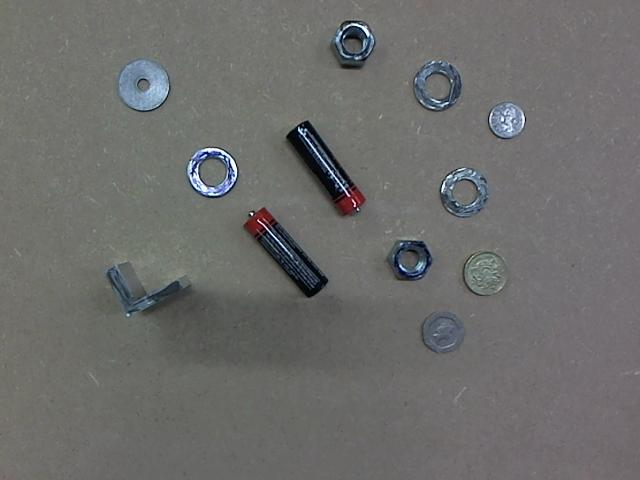
\includegraphics[width=\textwidth]{./img/sample_fig/02.jpg}
  \end{subfigure}
  \begin{subfigure}[b]{.3\textwidth}
    \centering
    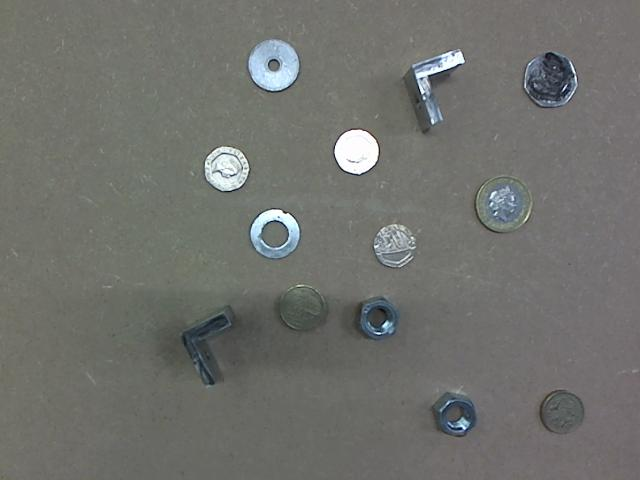
\includegraphics[width=\textwidth]{./img/sample_fig/04.jpg}
  \end{subfigure}
  \begin{subfigure}[b]{.3\textwidth}
    \centering
    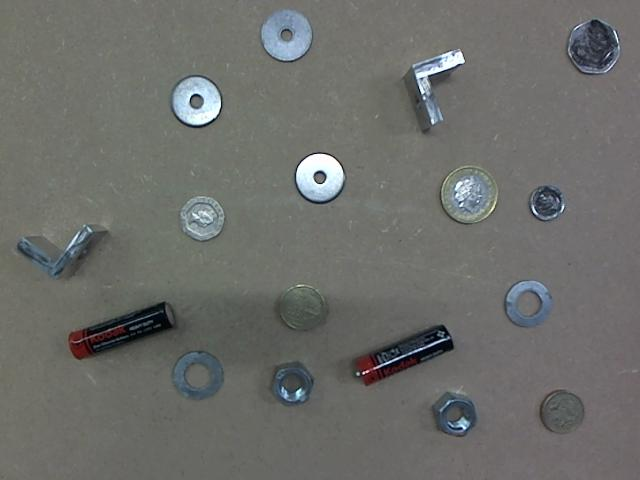
\includegraphics[width=\textwidth]{./img/sample_fig/03.jpg}
  \end{subfigure}
  \caption{Sample images from given data.}
  \label{montage_data}
\end{figure}
\begin{figure}[!h]
  \centering
  \begin{subfigure}[b]{.3\textwidth}
    \centering
    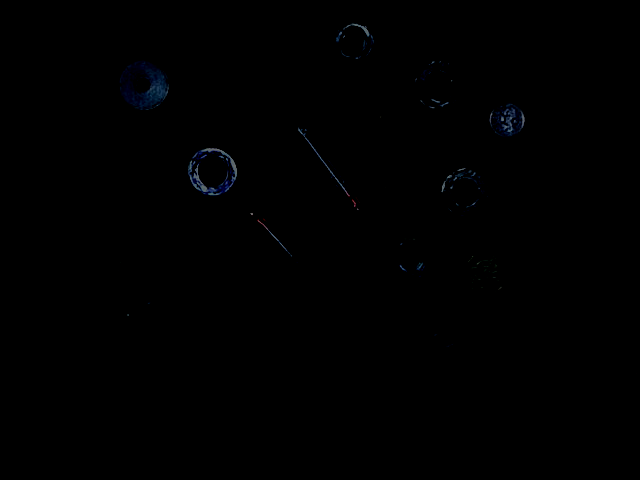
\includegraphics[width=\textwidth]{./img/bg_model/02_bgremove.png}
  \end{subfigure}
  \begin{subfigure}[b]{.3\textwidth}
    \centering
    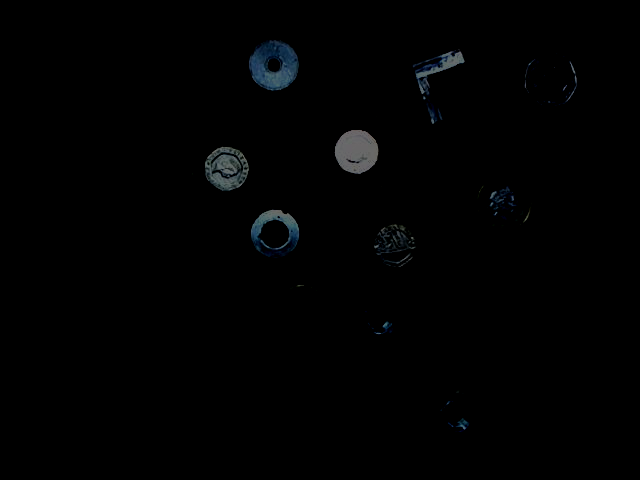
\includegraphics[width=\textwidth]{./img/bg_model/04_bgremove.png}
  \end{subfigure}
  \begin{subfigure}[b]{.3\textwidth}
    \centering
    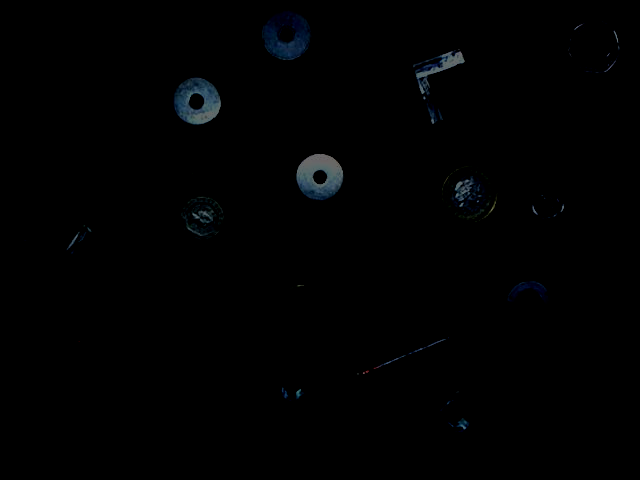
\includegraphics[width=\textwidth]{./img/bg_model/03_bgremove.png}
  \end{subfigure}
  \caption{Sample images after their background is subtracted.}
  \label{montage_data_bgremove}
\end{figure}


\subsection*{Image Processing}
The image processing step aims to 1) make all images (for training the model or for evaluation) comparable, 2) extract objects in the foreground (also known as image segmentation). The outcome of this stage is an array of subimages ready for feature extraction.

The central idea is to, first, model the background before subtracting it from all images; second - make the edges of the objects 'obvious' by finding a suitable threshold to binarise the image; third - crop out the objects to obtain the subimages, which will be our data points.

\subsection*{Feaure Extraction}
Given the subimages, this stage aims to represent each subimages with a feature vector that contains properties to adequately describe the class it belongs to (or shape). Notaby, we have many circular objects varying in size. This renders global descriptors such as convexity and elongation less useful for these classes.

\subsection*{Classification}
The task here is to label an unknown (sub)image given its set of feature vector. The model we consider is a multivarate gaussian classifier that classify an image based on the parameters of each class (class mean and standard deviation (or variance)). This multivarate gaussian classifier outputs the posterior probability of a given feature vector $x$ ($P(C_{k}|X)$) for each class $k$, with the class giving the highest probability being the label. That is $x.class = argmax_{k} P(C_{k}|x)$.

A slight tweak for Coinsy is her ability to reject the class label output by the classifier if the highest probability falls out of her confidence interval. In such cases, Coinsy will intervene and change the class to unknown (class 11).

The last step of Coinsy is to sum the value of all the objects she managed to identify from a given image.

\subsection*{Code}
The following directory trees will provide an overview of the code utilitsed for the project. Codes presented in the appendix are hyperlinked, although some may depend on the code repository given in \url{http://www.inf.ed.ac.uk/teaching/courses/ivr/matlab/flatpartrecog/}.

\dirtree{%
  .1 src.
  .2 imgs\DTcomment{Store images from function}.
  .2 dataset\DTcomment{Datasets from experiments}.
  .2 \hyperlink{setup}{setup}.
  .2 \hyperlink{training}{training}.
  .2 \hyperlink{main}{main}.
  .2 \hyperlink{imageprocessing}{image\_processing}.
  .2 \hyperlink{gradmag}{gradmag\_edge}.
  .2 \hyperlink{extractfeat}{extract\_features}.
  .2 \hyperlink{manclf}{manual\_classification}.
  .2 \hyperlink{trainclf}{trainclf\_loglikelihood}.
  .2 filters.
  .3 \hyperlink{medianfilter}{median\_filter}.
  .3 \hyperlink{medianfiliter}{median\_filter\_iter}.
  .3 \hyperlink{gaussfilter}{gaussian\_filter\_1d}.
  .3 \hyperlink{gauss2d}{gaussian\_filter\_2d}.
  .3
  .2 image\_processing.
  .3 \hyperlink{normRGB}{normalise\_RGB}.
  .3 \hyperlink{bgextract}{bg\_extract}.
  .3 \hyperlink{bgsub}{bg\_subtraction}.
  .3 \hyperlink{dothresh}{dothresh}.
  .3 \hyperlink{edgemorphdisk}{edg\_morph\_disk}.
  .2 features.
  .3 \hyperlink{getfeatures}{getFeatures}.
  .3 \hyperlink{rawmoment}{rawmmoment}.
  .3 \hyperlink{centralmoment}{centralmoment}.
  .3 \hyperlink{simoment}{SI\_moment}.
  .3 \hyperlink{humoment}{humomentinvariants}.
  .3 \hyperlink{complex}{complexmoment}.
  .2 classification.
  .3 \hyperlink{splitdata}{split\_data}.
  .3 \hyperlink{userclf}{user\_classify}.
  .3 \hyperlink{findconf}{findConfusion}.
  .3 \hyperlink{gaussianDist}{gaussianDistr}.
  .3 \hyperlink{gaussianclf}{multivarate}.
}

\end{document}
